% Generated by build_report.py; shared quantitative PublicCover architecture.
\subsection{Nhánh PublicCover: CoverLite-30 và CoverPlus-67}
\textbf{Hai cấu hình của cùng nhánh bảo vệ dịch vụ:} CoverLite-30 giảm số truy vấn; CoverPlus-67 tăng độ phủ POI. Kế hoạch được lập từ bản đồ/danh mục công khai trước khi đọc chuyến đánh giá. Nhánh này không dùng neo Geo-I; số 30/67 đếm cặp loại POI–tọa độ, không phải K dummy hay ngân sách $\varepsilon$. Greedy chọn từng cặp có tỷ lệ POI mới lớn nhất trong loại; 67 là số thu được trên danh mục hiện tại.

\begin{center}
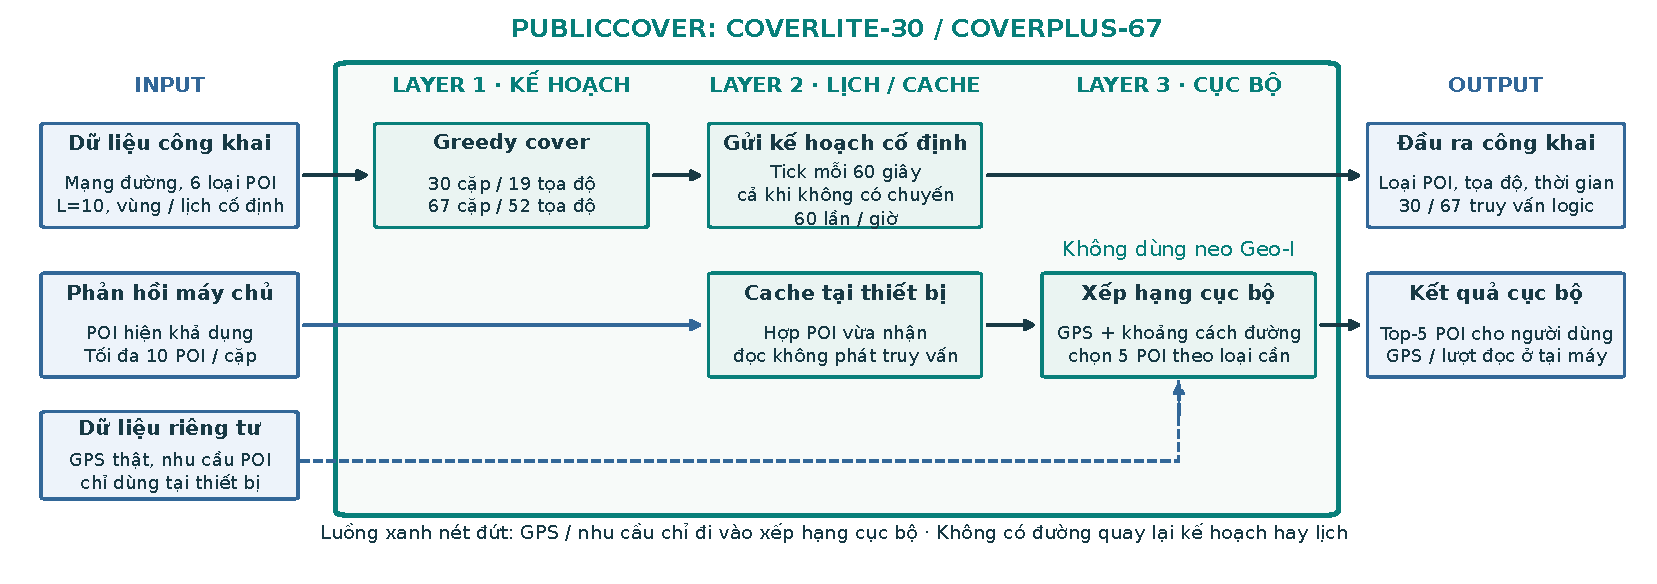
\includegraphics[width=\linewidth]{figures/architecture_publiccover.pdf}
\end{center}
Khung xanh là PublicCover tại thiết bị. Layer 1 lập kế hoạch cố định; layer 2 gửi theo lịch và lưu phản hồi; layer 3 dùng GPS để chọn top-5 cục bộ. GPS và lúc dùng dịch vụ không điều khiển kế hoạch hoặc lịch đã đăng ký.

\begingroup\small
\begin{longtable}{@{}P{5.612cm}P{5.513cm}P{5.513cm}@{}}
\toprule
\textbf{Thông số / kết quả} & \textbf{CoverLite-30} & \textbf{CoverPlus-67}\\\midrule
\endfirsthead
\toprule
\textbf{Thông số / kết quả} & \textbf{CoverLite-30} & \textbf{CoverPlus-67}\\\midrule
\endhead
\bottomrule\endfoot
Cách chọn kế hoạch & Greedy, dừng ở ngân sách 30 & Greedy đến khi không tăng độ phủ; được 67\\
\addlinespace[3pt]
Truy vấn logic / lần gửi & 30 cặp loại POI–tọa độ & 67 cặp loại POI–tọa độ\\
\addlinespace[3pt]
Tọa độ khác nhau & 19 & 52\\
\addlinespace[3pt]
POI tĩnh nằm trong hợp phản hồi & 259/419; thiếu 160 & 411/419; thiếu 8\\
\addlinespace[3pt]
Lượt POI trả về tối đa / lần & $\le$300 (30 $\times$ L=10) & $\le$670 (67 $\times$ L=10)\\
\addlinespace[3pt]
Lịch endpoint: 60 lần gửi / giờ & 1.800 truy vấn logic / giờ & 4.020 truy vấn logic / giờ\\
\addlinespace[3pt]
Recall@5 tại p=0,8; ca đạt $\ge$90\% & 95,00\%; 14/14 & 100,00\%; 14/14\\
\addlinespace[3pt]
Recall@5 tại p=0,95; ca đạt $\ge$90\% & 93,01\%; 13/14 & 100,00\%; 14/14\\
\addlinespace[3pt]
Hit100 S9 / S10; lịch, 32 nhóm & 0,00\% / 0,00\% & 0,00\% / 0,00\%\\
\addlinespace[3pt]
Byte gửi + nhận / sự kiện dịch vụ & 3.071,0 & 6.878,6\\
\end{longtable}
\endgroup
\textbf{Đọc số liệu:} độ phủ tĩnh chấm 419 POI mục tiêu; Recall chấm top-5 của mẫu chuyến. Lượt phản hồi có thể trùng POI. Cả hai hỏi đủ sáu loại: cafe, clinic, fuel, hospital, pharmacy, restaurant; máy chủ trả tối đa L=10 mỗi cặp, thiết bị chọn k=5. Các hàng Recall/Hit/byte dùng kết quả 32 nhóm với lịch công khai, p là tỷ lệ POI khả dụng; byte gồm traffic ngoài chuyến, chưa gồm HTTP/TLS. Lịch là [0, 3.600) giây, tick mỗi 60 giây; số truy vấn/giờ là phép đếm từ cấu hình, không phải số gói HTTP.

\key{Lite và Plus chủ yếu là đánh đổi độ phủ dịch vụ–chi phí. Hai cấu hình cùng có Hit100=0 trong phép thử S9/S10; chưa chứng minh Plus riêng tư hơn Lite. Che giờ chuyến đến từ lịch cố định; bảo vệ có điều kiện vùng/lịch đăng ký trước, không bao gồm IP, account hoặc click. Plus vẫn thiếu 8 POI tĩnh dù Recall trên mẫu đạt 100\%.}

